\begin{frame}{Languages recap}
  
  \begin{description}[Turing machine]
    \setlength\itemsep{5mm}
    \item[Alphabet] is a set usually denoted \( A \). \\ e.g. \( A = \{ 0 , 1 \} \)
    \item[Kleene star] of a an alphabet is all strings over it. \\ e.g. \( A^* = \{ \epsilon, 0, 1, 00, 01, \ldots \} \)
    \item[Language] is a subset of the Kleene star of an alphabet. \\  e.g. \( L = \{ 10, 11, 101, 111, 1011, \ldots \} \subseteq A^* \)
    \item[Turing machine] accepts a language. It decides if it always halts.
  \end{description}

\end{frame}

\begin{frame}{TIME}
  
  \red{\(TIME(f(n))\) is the set of languages with an \(O(n^k)\) decider.}

  \begin{description}
    \setlength\itemsep{2mm}
    \item[Denote] by \(n\) the length (\(\in \mathbb{N}\)) of an input string to a decider (Turing machine that always halts).
    \item[Calculate] the maximum number of state table lookups a given decider takes to halt in terms of \(n\).
    \item[One way] to do this is calculate the value for \(n=0\), \(n=1\), \(n=2\), \(n=3\), and so on, and try to generalise.
    \item[Find] a succinct function \(f(n)\) that bounds it beyond a fixed value of \(n\). Then we say the decider is \(O(f)\). Note that deciders are \(O(g)\) for lots of functions \(g\).
  \end{description}

\end{frame}


\begin{frame}[fragile]{Big-O}
  \begin{center}
    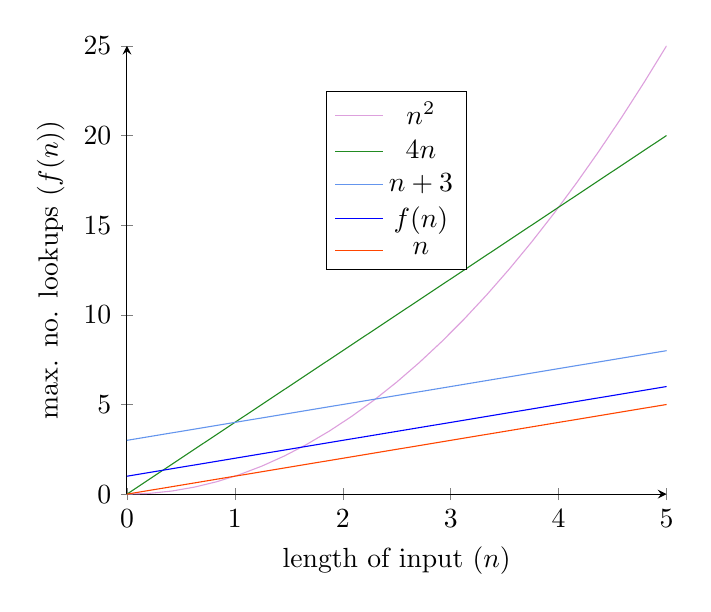
\begin{tikzpicture}
      \begin{axis}[xmin=0, domain=0:5, axis x line=bottom, axis y line=left, legend style={at={(0.5,0.5)},anchor=south}, xlabel={length of input (\(n\))}, ylabel={max. no. lookups (\(f(n)\))}]
        \addplot[Plum]           {pow(x,2)};
        \addplot[ForestGreen]    {4*x};
        \addplot[CornflowerBlue] {x+3};
        \addplot[Blue]           {x+1};
        \addplot[OrangeRed]      {x};
        \legend{\(n^2\),\(4n\),\(n+3\),\(f(n)\),\(n\)};
      \end{axis}
    \end{tikzpicture}
  \end{center}
\end{frame}


\begin{frame}{Polynomial time}
  
  \redmath{P = \bigcup_k \text{TIME}(n^k)}
  
  \begin{description}
    \item[Decidable] languages are languages for which there is at least one Turing machine that halts in a finite number of state table lookups for each input.
    \item[P] is the set of languages that are decidable in polynomial time using a deterministic Turing machine.
    \item[Polynomial] means that for a length of input \( n \) the number of steps (state table lookups) is \( O(n^k) \) for some \( k \in \mathbb{N} \).
    \item[\( \text{TIME}(n^k) \)] is the set of languages decidable in \( O(n^k) \) steps.
  \end{description}

\end{frame}


\begin{frame}[fragile]{Recap on polynomials}
  
  \redmath{a_0 + a_1 x + a_2 x^2 + \cdots + a_m x^m \text{ where } a_i \in \mathbb{R}, m \in \mathbb{N}}
  
  \begin{description}
    \item[Polynomials] have a fixed number of operations (add, multiply) to perform for all values of \( x \).
    \item[Exponential] contrasts with polynomial, having a variable number of operations, e.g. \( 2^x \).
    \item[Functions] that are polynomial in $n$ are functions that take $n$ and plug it into a polynomial to give the result.
  \end{description}

  \begin{adjustbox}{max width={0.4\textwidth}, center}
    \begin{tikzpicture}
      \begin{axis}[xmin=0, domain=0:3, axis x line=bottom, axis y line=left, legend style={at={(0.4,0.4)},anchor=south}]
        \addplot[black] {pow(x,4) + 5*pow(x, 2) + 1};
        \legend{$x^4 + 5 x^2 + 1$};
      \end{axis}
    \end{tikzpicture}
  \end{adjustbox}

\end{frame}


\begin{frame}[fragile]{Polynomials are closed}
  
  \redmath{\mathbb{R}[x] = \{ a_0 + a_1 x + a_2 x^2 + \cdots + a_m x^m \mid a_i \in \mathbb{R}, m \in \mathbb{N} \}}
  
  The set of all polynomials is closed under the following operations:
  \begin{description}[Multiplication:]
    \setlength\itemsep{4mm}
    \item[Addition:] \( (x^4 + 1) + (5 x^3 + x) = x^4 + 5 x^3 + x + 1 \)
    \item[Multiplication:] \( (x^4 + 1) \times (5 x^3 + x) = 5 x^7 + x^5 + 5 x^3 + x \)
    \item[Composition:] \( ((5 x^3 + x))^4 + 1  = 625x^{12} + 500 x^{10} + 150x^8 + 20x^6 + x^4 +1 \)
  \end{description}

  \red{Applying two polynomial time algorithms one after the other is still polynomial time.}

\end{frame}


\begin{frame}{Tractability}
  
  \begin{description}
    \item[Cobham's] thesis is that P represents the tractable problems.
    \item[Operations] $+$, $-$, $\times$ and $\div$ are \(O(n^k)\).
    \item[Space] -- a decider for a problem in P cannot move more than a polynomial number of steps along the tape.
    \item[Exponential time] is a superset of polynomial time.
    \item[Subexponential] means the language is in a complexity class less than exponential time.
    \item[Strictly] exponential time problems are considered intractable.
    \item[Careful:] would you consider a language whose best known decider is $O(n^{100000})$ tractable?
  \end{description}

  \red{The exponential time hypothesis is that 3-SAT can't be solved in subexponential time. 3-SAT is NP-complete.}

\end{frame}

